Here we will use the corrections for different types of Hamiltonian and different eSTA protocols to check how the fidelity is affected by this conditions.
In particular we will use various number of particles to assess the improvement.

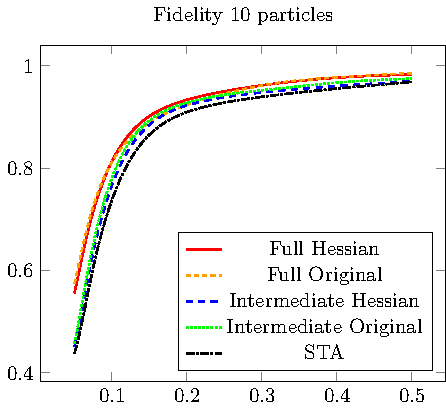
\includegraphics{./gfx/fidelity_np10_nlambda5.pdf}
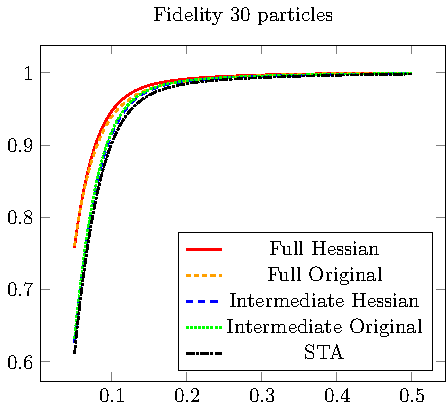
\includegraphics{./gfx/fidelity_np30_nlambda5.pdf}

\begin{center}
    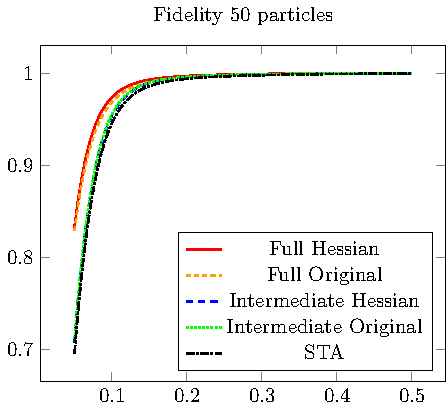
\includegraphics{./gfx/fidelity_np50_nlambda5.pdf}
\end{center}


As we can see, the best performances are achieved by the Hessian version eSTA protocol.
The fidelities are calculated using 5 $ \lambda $, in the following we will compare the fidelity for different number of corrections.
Since the behaviour of the fidelity is roughly the same regardless of the number of particles, in the following we will focus only on 10 particles as it is the most extreme case.
Moreover, we will use only the protocol that yields the best performance so in this case we will use the eSTA corrections evaluated from the original Hamiltonian and with the Hessian formalism.

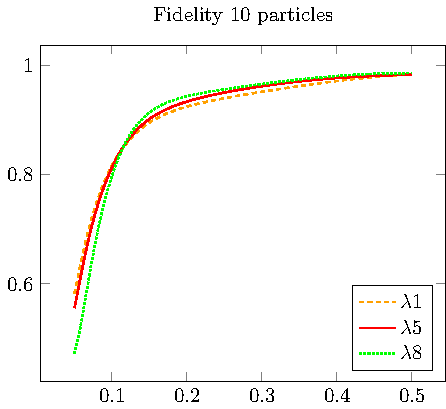
\includegraphics{./gfx/fidelity_compare10.pdf}
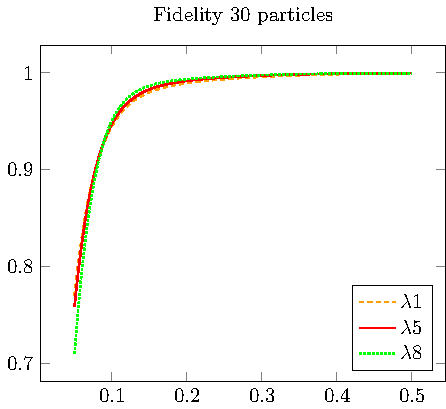
\includegraphics{./gfx/fidelity_compare30.pdf}

\begin{center}
    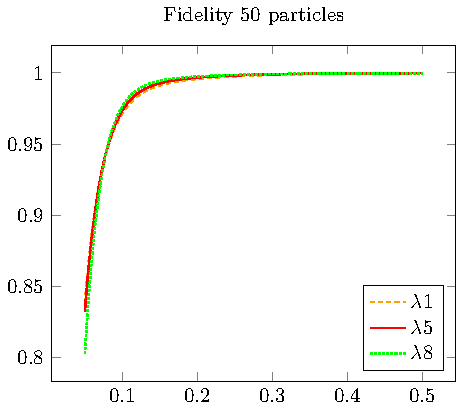
\includegraphics{./gfx/fidelity_compare50.pdf}
\end{center}
